% Options for packages loaded elsewhere
% Options for packages loaded elsewhere
\PassOptionsToPackage{unicode}{hyperref}
\PassOptionsToPackage{hyphens}{url}
%
\documentclass[
  indonesian,
  letterpaper,
  DIV=11,
  numbers=noendperiod]{scrartcl}
\usepackage{xcolor}
\usepackage{amsmath,amssymb}
\setcounter{secnumdepth}{-\maxdimen} % remove section numbering
\usepackage{iftex}
\ifPDFTeX
  \usepackage[T1]{fontenc}
  \usepackage[utf8]{inputenc}
  \usepackage{textcomp} % provide euro and other symbols
\else % if luatex or xetex
  \usepackage{unicode-math} % this also loads fontspec
  \defaultfontfeatures{Scale=MatchLowercase}
  \defaultfontfeatures[\rmfamily]{Ligatures=TeX,Scale=1}
\fi
\usepackage{lmodern}
\ifPDFTeX\else
  % xetex/luatex font selection
\fi
% Use upquote if available, for straight quotes in verbatim environments
\IfFileExists{upquote.sty}{\usepackage{upquote}}{}
\IfFileExists{microtype.sty}{% use microtype if available
  \usepackage[]{microtype}
  \UseMicrotypeSet[protrusion]{basicmath} % disable protrusion for tt fonts
}{}
\makeatletter
\@ifundefined{KOMAClassName}{% if non-KOMA class
  \IfFileExists{parskip.sty}{%
    \usepackage{parskip}
  }{% else
    \setlength{\parindent}{0pt}
    \setlength{\parskip}{6pt plus 2pt minus 1pt}}
}{% if KOMA class
  \KOMAoptions{parskip=half}}
\makeatother
% Make \paragraph and \subparagraph free-standing
\makeatletter
\ifx\paragraph\undefined\else
  \let\oldparagraph\paragraph
  \renewcommand{\paragraph}{
    \@ifstar
      \xxxParagraphStar
      \xxxParagraphNoStar
  }
  \newcommand{\xxxParagraphStar}[1]{\oldparagraph*{#1}\mbox{}}
  \newcommand{\xxxParagraphNoStar}[1]{\oldparagraph{#1}\mbox{}}
\fi
\ifx\subparagraph\undefined\else
  \let\oldsubparagraph\subparagraph
  \renewcommand{\subparagraph}{
    \@ifstar
      \xxxSubParagraphStar
      \xxxSubParagraphNoStar
  }
  \newcommand{\xxxSubParagraphStar}[1]{\oldsubparagraph*{#1}\mbox{}}
  \newcommand{\xxxSubParagraphNoStar}[1]{\oldsubparagraph{#1}\mbox{}}
\fi
\makeatother

\usepackage{color}
\usepackage{fancyvrb}
\newcommand{\VerbBar}{|}
\newcommand{\VERB}{\Verb[commandchars=\\\{\}]}
\DefineVerbatimEnvironment{Highlighting}{Verbatim}{commandchars=\\\{\}}
% Add ',fontsize=\small' for more characters per line
\usepackage{framed}
\definecolor{shadecolor}{RGB}{241,243,245}
\newenvironment{Shaded}{\begin{snugshade}}{\end{snugshade}}
\newcommand{\AlertTok}[1]{\textcolor[rgb]{0.68,0.00,0.00}{#1}}
\newcommand{\AnnotationTok}[1]{\textcolor[rgb]{0.37,0.37,0.37}{#1}}
\newcommand{\AttributeTok}[1]{\textcolor[rgb]{0.40,0.45,0.13}{#1}}
\newcommand{\BaseNTok}[1]{\textcolor[rgb]{0.68,0.00,0.00}{#1}}
\newcommand{\BuiltInTok}[1]{\textcolor[rgb]{0.00,0.23,0.31}{#1}}
\newcommand{\CharTok}[1]{\textcolor[rgb]{0.13,0.47,0.30}{#1}}
\newcommand{\CommentTok}[1]{\textcolor[rgb]{0.37,0.37,0.37}{#1}}
\newcommand{\CommentVarTok}[1]{\textcolor[rgb]{0.37,0.37,0.37}{\textit{#1}}}
\newcommand{\ConstantTok}[1]{\textcolor[rgb]{0.56,0.35,0.01}{#1}}
\newcommand{\ControlFlowTok}[1]{\textcolor[rgb]{0.00,0.23,0.31}{\textbf{#1}}}
\newcommand{\DataTypeTok}[1]{\textcolor[rgb]{0.68,0.00,0.00}{#1}}
\newcommand{\DecValTok}[1]{\textcolor[rgb]{0.68,0.00,0.00}{#1}}
\newcommand{\DocumentationTok}[1]{\textcolor[rgb]{0.37,0.37,0.37}{\textit{#1}}}
\newcommand{\ErrorTok}[1]{\textcolor[rgb]{0.68,0.00,0.00}{#1}}
\newcommand{\ExtensionTok}[1]{\textcolor[rgb]{0.00,0.23,0.31}{#1}}
\newcommand{\FloatTok}[1]{\textcolor[rgb]{0.68,0.00,0.00}{#1}}
\newcommand{\FunctionTok}[1]{\textcolor[rgb]{0.28,0.35,0.67}{#1}}
\newcommand{\ImportTok}[1]{\textcolor[rgb]{0.00,0.46,0.62}{#1}}
\newcommand{\InformationTok}[1]{\textcolor[rgb]{0.37,0.37,0.37}{#1}}
\newcommand{\KeywordTok}[1]{\textcolor[rgb]{0.00,0.23,0.31}{\textbf{#1}}}
\newcommand{\NormalTok}[1]{\textcolor[rgb]{0.00,0.23,0.31}{#1}}
\newcommand{\OperatorTok}[1]{\textcolor[rgb]{0.37,0.37,0.37}{#1}}
\newcommand{\OtherTok}[1]{\textcolor[rgb]{0.00,0.23,0.31}{#1}}
\newcommand{\PreprocessorTok}[1]{\textcolor[rgb]{0.68,0.00,0.00}{#1}}
\newcommand{\RegionMarkerTok}[1]{\textcolor[rgb]{0.00,0.23,0.31}{#1}}
\newcommand{\SpecialCharTok}[1]{\textcolor[rgb]{0.37,0.37,0.37}{#1}}
\newcommand{\SpecialStringTok}[1]{\textcolor[rgb]{0.13,0.47,0.30}{#1}}
\newcommand{\StringTok}[1]{\textcolor[rgb]{0.13,0.47,0.30}{#1}}
\newcommand{\VariableTok}[1]{\textcolor[rgb]{0.07,0.07,0.07}{#1}}
\newcommand{\VerbatimStringTok}[1]{\textcolor[rgb]{0.13,0.47,0.30}{#1}}
\newcommand{\WarningTok}[1]{\textcolor[rgb]{0.37,0.37,0.37}{\textit{#1}}}

\usepackage{longtable,booktabs,array}
\usepackage{calc} % for calculating minipage widths
% Correct order of tables after \paragraph or \subparagraph
\usepackage{etoolbox}
\makeatletter
\patchcmd\longtable{\par}{\if@noskipsec\mbox{}\fi\par}{}{}
\makeatother
% Allow footnotes in longtable head/foot
\IfFileExists{footnotehyper.sty}{\usepackage{footnotehyper}}{\usepackage{footnote}}
\makesavenoteenv{longtable}
\usepackage{graphicx}
\makeatletter
\newsavebox\pandoc@box
\newcommand*\pandocbounded[1]{% scales image to fit in text height/width
  \sbox\pandoc@box{#1}%
  \Gscale@div\@tempa{\textheight}{\dimexpr\ht\pandoc@box+\dp\pandoc@box\relax}%
  \Gscale@div\@tempb{\linewidth}{\wd\pandoc@box}%
  \ifdim\@tempb\p@<\@tempa\p@\let\@tempa\@tempb\fi% select the smaller of both
  \ifdim\@tempa\p@<\p@\scalebox{\@tempa}{\usebox\pandoc@box}%
  \else\usebox{\pandoc@box}%
  \fi%
}
% Set default figure placement to htbp
\def\fps@figure{htbp}
\makeatother



\ifLuaTeX
\usepackage[bidi=basic,provide=*]{babel}
\else
\usepackage[bidi=default,provide=*]{babel}
\fi
% get rid of language-specific shorthands (see #6817):
\let\LanguageShortHands\languageshorthands
\def\languageshorthands#1{}


\setlength{\emergencystretch}{3em} % prevent overfull lines

\providecommand{\tightlist}{%
  \setlength{\itemsep}{0pt}\setlength{\parskip}{0pt}}



 


\KOMAoption{captions}{tableheading}
\makeatletter
\@ifpackageloaded{caption}{}{\usepackage{caption}}
\AtBeginDocument{%
\ifdefined\contentsname
  \renewcommand*\contentsname{Daftar Isi}
\else
  \newcommand\contentsname{Daftar Isi}
\fi
\ifdefined\listfigurename
  \renewcommand*\listfigurename{Daftar Gambar}
\else
  \newcommand\listfigurename{Daftar Gambar}
\fi
\ifdefined\listtablename
  \renewcommand*\listtablename{Daftar Tabel}
\else
  \newcommand\listtablename{Daftar Tabel}
\fi
\ifdefined\figurename
  \renewcommand*\figurename{Gambar}
\else
  \newcommand\figurename{Gambar}
\fi
\ifdefined\tablename
  \renewcommand*\tablename{Tabel}
\else
  \newcommand\tablename{Tabel}
\fi
}
\@ifpackageloaded{float}{}{\usepackage{float}}
\floatstyle{ruled}
\@ifundefined{c@chapter}{\newfloat{codelisting}{h}{lop}}{\newfloat{codelisting}{h}{lop}[chapter]}
\floatname{codelisting}{Daftar}
\newcommand*\listoflistings{\listof{codelisting}{Daftar Daftar}}
\makeatother
\makeatletter
\makeatother
\makeatletter
\@ifpackageloaded{caption}{}{\usepackage{caption}}
\@ifpackageloaded{subcaption}{}{\usepackage{subcaption}}
\makeatother
\usepackage{bookmark}
\IfFileExists{xurl.sty}{\usepackage{xurl}}{} % add URL line breaks if available
\urlstyle{same}
\hypersetup{
  pdflang={id-ID},
  hidelinks,
  pdfcreator={LaTeX via pandoc}}


\author{}
\date{}
\begin{document}


\begin{titlepage}
\begin{center}

\vspace*{1cm}

{\Large \textbf{PENGARUH PENETRASI AKSES INTERNET TERHADAP}}\\
{\Large \textbf{INDEKS PEMBANGUNAN MANUSIA (IPM):}}\\
{\Large \textbf{PENDEKATAN PROBABILITAS DAN ANALISIS KORELASI}}\\[1.2cm]


\includegraphics[width=3.5cm]{../gambar/ipb.png}\\[1cm]

\textbf{Mata Kuliah:}\\
Probabilitas dan Statistika\\[0.8cm]

\textbf{Disusun oleh:}\\[0.3cm]
Alfitra Mumtaz Hanafi (J0403251058)\\
Ahmad Abian Hakim (J0403251069)\\
Rheika Muhammad Dzikrulhakim (J0403251068)\\
Zaky Alnadif (J0403251126)\\
Natasha Umaiza (J0403251046)\\
Hilannisa Nuraini Al'Basr (J0403251022)\\[1cm]

\textbf{TEKNOLOGI REKAYASA PERANGKAT LUNAK}\\
\textbf{SEKOLAH VOKASI}\\
\textbf{IPB UNIVERSITY}\\
\textbf{BOGOR}\\
\textbf{2026}

\end{center}
\end{titlepage}

\newpage

\renewcommand{\contentsname}{Daftar Isi}
\tableofcontents

\newpage

\section{BAB I: PENDAHULUAN}\label{bab-i-pendahuluan}

\subsection{1.1 Latar Belakang}\label{latar-belakang}

Dalam era modern, definisi infrastruktur pembangunan tidak lagi terbatas
pada pembangunan fisik, melainkan telah berekspansi ke infrastruktur
digital. Akses internet kini menjadi salah satu fasilitas penting yang
berperan dalam mendukung akses informasi, pendidikan, layanan publik,
dan aktivitas ekonomi masyarakat. Kesenjangan digital (\emph{digital
divide}) sering kali menjadi salah satu faktor yang berkaitan dengan
ketimpangan pembangunan antarwilayah (Ndubuisi et al., 2021).

Indeks Pembangunan Manusia (IPM) digunakan untuk melihat capaian
pembangunan manusia dari aspek kesehatan, pendidikan, dan standar hidup
layak. Konsep ini menunjukkan bahwa pembangunan tidak hanya diukur dari
pertumbuhan ekonomi, tetapi juga dari kualitas hidup masyarakat secara
lebih luas (UNDP, 2022). Oleh karena itu, analisis ini dilakukan untuk
melihat apakah tingkat akses internet memiliki hubungan linear yang
signifikan dengan IPM pada dataset pembangunan wilayah yang digunakan.

\subsection{1.2 Rumusan Masalah}\label{rumusan-masalah}

Berdasarkan latar belakang tersebut, rumusan masalah dalam analisis ini
adalah:

\begin{enumerate}
\def\labelenumi{\arabic{enumi}.}
\tightlist
\item
  Bagaimana kondisi missing value dan outlier pada dataset pembangunan
  wilayah?
\item
  Bagaimana gambaran statistik deskriptif variabel akses internet dan
  IPM?
\item
  Bagaimana pola visual hubungan antara akses internet dan IPM?
\item
  Apakah data IPM berdistribusi normal?
\item
  Apakah terdapat hubungan linear yang signifikan antara akses internet
  dan IPM?
\end{enumerate}

\subsection{1.3 Tujuan Analisis}\label{tujuan-analisis}

Analisis ini memiliki tujuan antara lain:

\begin{enumerate}
\def\labelenumi{\arabic{enumi}.}
\tightlist
\item
  Mengidentifikasi dan menangani \emph{missing value} serta
  \emph{outlier} pada dataset pembangunan wilayah, khususnya pada
  variabel akses internet dan IPM.
\item
  Melakukan statistika deskriptif untuk memetakan persebaran data
  digitalisasi dan kesejahteraan penduduk.
\item
  Membangun visualisasi data yang informatif untuk melihat tren sebaran
  antarvariabel secara grafis.
\item
  Menguji distribusi probabilitas atau normalitas pada data IPM wilayah.
\item
  Membuktikan secara statistik hipotesis korelasi antara penetrasi akses
  internet dengan skor IPM.
\end{enumerate}

\subsection{1.4 Manfaat Analisis}\label{manfaat-analisis}

Analisis ini diharapkan dapat memberikan gambaran mengenai proses
pengolahan dataset pembangunan wilayah menggunakan R, mulai dari
pemeriksaan kualitas data, statistika deskriptif, visualisasi, pengujian
distribusi, hingga analisis korelasi. Selain itu, hasil analisis ini
dapat menjadi bahan awal untuk memahami apakah akses internet memiliki
hubungan linear dengan IPM pada dataset yang digunakan.

\section{BAB II: METODOLOGI}\label{bab-ii-metodologi}

\subsection{2.1 Dataset}\label{dataset}

Penelitian ini menggunakan dataset
\texttt{pembangunan\_wilayah\_missing\_outlier.csv} yang
merepresentasikan kondisi indikator pembangunan makro di berbagai
wilayah. Fokus pengujian dibatasi pada variabel independen
\texttt{akses\_internet} (persentase ketersediaan fasilitas internet)
dan variabel dependen \texttt{ipm} (Indeks Pembangunan Manusia). Dataset
ini secara inheren memiliki \emph{missing value} dan \emph{outlier} yang
disimulasikan untuk menguji ketahanan model pra-pemrosesan data sebelum
uji hipotesis dieksekusi.

\subsection{2.2 Tools yang Digunakan}\label{tools-yang-digunakan}

Seluruh tahapan pembersihan dan pengujian data dieksekusi menggunakan
bahasa pemrograman \textbf{R}. R digunakan karena mendukung proses
komputasi statistik, eksplorasi data, dan visualisasi secara sistematis
(Field et al., 2012). Dokumen ini disusun menggunakan \textbf{Quarto},
yaitu sistem penulisan yang memungkinkan integrasi narasi, kode, dan
output analisis dalam satu laporan yang dapat direproduksi. Pustaka
tambahan seperti \texttt{ggplot2} digunakan untuk membangun visualisasi
grafis yang lebih informatif.

\subsection{2.3 Metode Analisis}\label{metode-analisis}

Pendekatan statistik yang diterapkan meliputi:

\begin{itemize}
\item
  \textbf{Penanganan Data:} Imputasi data kosong diselesaikan
  menggunakan Median Imputation. Metode ini dipilih karena median lebih
  tahan terhadap pengaruh nilai ekstrem atau outlier dibandingkan
  rata-rata, sehingga lebih sesuai digunakan ketika dataset memiliki
  potensi nilai ekstrem (Little \& Rubin, 2019). Karena fokus penelitian
  adalah menguji hubungan antara \textbf{akses internet dan IPM},
  analisis selanjutnya dilakukan menggunakan data hasil imputasi pada
  variabel utama tanpa menghapus observasi yang terindikasi sebagai
  nilai ekstrem.
\item
  \textbf{Statistika Deskriptif:} Analisis deskriptif digunakan untuk
  melihat karakteristik awal variabel akses internet dan IPM, seperti
  nilai minimum, maksimum, median, rata-rata, dan kuartil.
\item
  \textbf{Visualisasi Data:} Visualisasi digunakan untuk membantu
  membaca kondisi missing value, catatan kualitas data, pola hubungan,
  distribusi IPM, serta kemungkinan adanya nilai ekstrem.
\item
  \textbf{Uji Normalitas:} Uji Shapiro-Wilk digunakan untuk melihat
  apakah data IPM mendekati distribusi normal.
\item
  \textbf{Uji Korelasi:} Uji korelasi Pearson digunakan untuk melihat
  kekuatan dan arah hubungan linear antara akses internet dan IPM.
\end{itemize}

\section{BAB III. HASIL DAN
PEMBAHASAN}\label{bab-iii.-hasil-dan-pembahasan}

\subsection{3.1 Gambaran Umum Analisis}\label{gambaran-umum-analisis}

Penelitian ini difokuskan untuk menguji apakah terdapat hubungan antara
penetrasi akses internet dengan Indeks Pembangunan Manusia (IPM).

Secara sistematis, prosedur analisis dilakukan dalam beberapa tahapan
krusial, dimulai dari persiapan data, eksplorasi deskriptif, visualisasi
pola hubungan antarvariabel, pengujian asumsi normalitas, hingga
diakhiri dengan uji korelasi. Mengingat dataset yang digunakan
mengandung missing value, langkah awal yang dilakukan adalah pembersihan
data untuk menjamin validitas hasil statistik. Setelah data dipastikan
lengkap, dilakukan eksplorasi untuk memetakan karakteristik variabel,
yang kemudian dilanjutkan dengan pengujian statistik untuk menjawab
hipotesis mengenai signifikansi hubungan antara akses internet dan IPM.~

\subsection{3.2 Pembersihan Data dan Penanganan Missing
Value}\label{pembersihan-data-dan-penanganan-missing-value}

Tahap awal dalam alur kerja analisis ini adalah memastikan integritas
data melalui pemeriksaan kualitas variabel. Keberadaan missing value
pada dataset berisiko menimbulkan bias dalam perhitungan statistik
sehingga diperlukan tindakan perbaikan sebelum analisis dilakukan. Untuk
menangani hal tersebut, metode Median Imputation diterapkan, yakni
mengganti nilai yang hilang dengan nilai median dari variabel terkait.
Pemilihan metode ini didasarkan pada karakteristik median yang lebih
resisten (\emph{robust}) terhadap pengaruh nilai ekstrem
(\emph{pencilan}) dibandingkan dengan metode rata-rata (\emph{mean}).~

Berdasarkan pemeriksaan awal, ditemukan adanya missing value pada
variabel akses internet dan IPM. Setelah proses imputasi dilakukan, data
kini telah lengkap dan memenuhi syarat untuk diproses ke tahap analisis
selanjutnya.

\subsubsection{3.2.1 Pemeriksaan Missing
Value}\label{pemeriksaan-missing-value}

\begin{Shaded}
\begin{Highlighting}[]
\CommentTok{\# Membuat folder gambar jika folder tersebut belum tersedia}
\ControlFlowTok{if}\NormalTok{ (}\SpecialCharTok{!}\FunctionTok{dir.exists}\NormalTok{(}\StringTok{"../gambar"}\NormalTok{)) \{}
  \FunctionTok{dir.create}\NormalTok{(}\StringTok{"../gambar"}\NormalTok{)}
\NormalTok{\}}

\CommentTok{\# Membaca dataset}
\NormalTok{data }\OtherTok{\textless{}{-}} \FunctionTok{read.csv}\NormalTok{(}\StringTok{"../dataset/pembangunan\_wilayah\_missing\_outlier.csv"}\NormalTok{)}

\CommentTok{\# Mengecek jumlah missing value pada seluruh variabel}
\NormalTok{missing\_semua\_variabel }\OtherTok{\textless{}{-}} \FunctionTok{colSums}\NormalTok{(}\FunctionTok{is.na}\NormalTok{(data))}

\FunctionTok{cat}\NormalTok{(}\StringTok{"Jumlah missing value pada seluruh variabel:}\SpecialCharTok{\textbackslash{}n}\StringTok{"}\NormalTok{)}
\end{Highlighting}
\end{Shaded}

\begin{verbatim}
Jumlah missing value pada seluruh variabel:
\end{verbatim}

\begin{Shaded}
\begin{Highlighting}[]
\FunctionTok{print}\NormalTok{(missing\_semua\_variabel)}
\end{Highlighting}
\end{Shaded}

\begin{verbatim}
          wilayah          provinsi             tahun    pdrb_perkapita 
                0                 0                 0                25 
       kemiskinan      pengangguran               ipm     harapan_hidup 
               24                25                25                 0 
rata_lama_sekolah    akses_internet        jalan_baik        air_bersih 
                0                25                25                 0 
     catatan_data 
                0 
\end{verbatim}

\begin{Shaded}
\begin{Highlighting}[]
\CommentTok{\# Mengecek jumlah missing value pada variabel utama}
\NormalTok{na\_internet\_awal }\OtherTok{\textless{}{-}} \FunctionTok{sum}\NormalTok{(}\FunctionTok{is.na}\NormalTok{(data}\SpecialCharTok{$}\NormalTok{akses\_internet))}
\NormalTok{na\_ipm\_awal }\OtherTok{\textless{}{-}} \FunctionTok{sum}\NormalTok{(}\FunctionTok{is.na}\NormalTok{(data}\SpecialCharTok{$}\NormalTok{ipm))}

\FunctionTok{cat}\NormalTok{(}\StringTok{"}\SpecialCharTok{\textbackslash{}n}\StringTok{Jumlah NA Akses Internet sebelum diolah:"}\NormalTok{, na\_internet\_awal, }\StringTok{"}\SpecialCharTok{\textbackslash{}n}\StringTok{"}\NormalTok{)}
\end{Highlighting}
\end{Shaded}

\begin{verbatim}

Jumlah NA Akses Internet sebelum diolah: 25 
\end{verbatim}

\begin{Shaded}
\begin{Highlighting}[]
\FunctionTok{cat}\NormalTok{(}\StringTok{"Jumlah NA IPM sebelum diolah:"}\NormalTok{, na\_ipm\_awal, }\StringTok{"}\SpecialCharTok{\textbackslash{}n}\StringTok{"}\NormalTok{)}
\end{Highlighting}
\end{Shaded}

\begin{verbatim}
Jumlah NA IPM sebelum diolah: 25 
\end{verbatim}

\begin{Shaded}
\begin{Highlighting}[]
\CommentTok{\# Mengisi missing value pada variabel utama dengan median}
\NormalTok{data}\SpecialCharTok{$}\NormalTok{akses\_internet[}\FunctionTok{is.na}\NormalTok{(data}\SpecialCharTok{$}\NormalTok{akses\_internet)] }\OtherTok{\textless{}{-}} \FunctionTok{median}\NormalTok{(data}\SpecialCharTok{$}\NormalTok{akses\_internet, }\AttributeTok{na.rm =} \ConstantTok{TRUE}\NormalTok{)}
\NormalTok{data}\SpecialCharTok{$}\NormalTok{ipm[}\FunctionTok{is.na}\NormalTok{(data}\SpecialCharTok{$}\NormalTok{ipm)] }\OtherTok{\textless{}{-}} \FunctionTok{median}\NormalTok{(data}\SpecialCharTok{$}\NormalTok{ipm, }\AttributeTok{na.rm =} \ConstantTok{TRUE}\NormalTok{)}

\CommentTok{\# Mengecek ulang missing value pada variabel utama setelah imputasi}
\FunctionTok{cat}\NormalTok{(}\StringTok{"}\SpecialCharTok{\textbackslash{}n}\StringTok{Jumlah NA Akses Internet setelah diolah:"}\NormalTok{, }\FunctionTok{sum}\NormalTok{(}\FunctionTok{is.na}\NormalTok{(data}\SpecialCharTok{$}\NormalTok{akses\_internet)), }\StringTok{"}\SpecialCharTok{\textbackslash{}n}\StringTok{"}\NormalTok{)}
\end{Highlighting}
\end{Shaded}

\begin{verbatim}

Jumlah NA Akses Internet setelah diolah: 0 
\end{verbatim}

\begin{Shaded}
\begin{Highlighting}[]
\FunctionTok{cat}\NormalTok{(}\StringTok{"Jumlah NA IPM setelah diolah:"}\NormalTok{, }\FunctionTok{sum}\NormalTok{(}\FunctionTok{is.na}\NormalTok{(data}\SpecialCharTok{$}\NormalTok{ipm)), }\StringTok{"}\SpecialCharTok{\textbackslash{}n}\StringTok{"}\NormalTok{)}
\end{Highlighting}
\end{Shaded}

\begin{verbatim}
Jumlah NA IPM setelah diolah: 0 
\end{verbatim}

Berdasarkan hasil pemeriksaan, missing value ditemukan pada beberapa
variabel dalam dataset. Namun, karena analisis ini berfokus pada
hubungan antara \texttt{akses\_internet} dan \texttt{ipm}, proses
imputasi hanya dilakukan pada kedua variabel tersebut. Nilai yang hilang
pada variabel \texttt{akses\_internet} dan \texttt{ipm} digantikan
menggunakan median masing-masing variabel sehingga data utama yang
digunakan dalam analisis menjadi lengkap.

\subsubsection{3.2.2 Pemeriksaan Outlier}\label{pemeriksaan-outlier}

\begin{Shaded}
\begin{Highlighting}[]
\CommentTok{\# Mengecek jumlah data berdasarkan catatan data}
\FunctionTok{cat}\NormalTok{(}\StringTok{"Jumlah data berdasarkan catatan\_data:}\SpecialCharTok{\textbackslash{}n}\StringTok{"}\NormalTok{)}
\end{Highlighting}
\end{Shaded}

\begin{verbatim}
Jumlah data berdasarkan catatan_data:
\end{verbatim}

\begin{Shaded}
\begin{Highlighting}[]
\FunctionTok{table}\NormalTok{(data}\SpecialCharTok{$}\NormalTok{catatan\_data)}
\end{Highlighting}
\end{Shaded}

\begin{verbatim}

Missing Value        Normal       Outlier 
          143          2337            20 
\end{verbatim}

Kolom \texttt{catatan\_data} menunjukkan bahwa sebagian observasi dalam
dataset teridentifikasi sebagai outlier, yakni nilai-nilai yang
menyimpang secara signifikan dari pola mayoritas data. Mengingat fokus
penelitian adalah menguji hubungan antara akses internet dan IPM,
observasi tersebut tetap dipertahankan dalam analisis. Penghapusan
outlier justru berisiko mempersempit variasi data dan mengurangi
representativitas hasil, sehingga pendekatan yang dipilih adalah
membiarkan data apa adanya setelah imputasi pada variabel utama
diselesaikan.

\subsection{3.3 Analisis Deskriptif}\label{analisis-deskriptif}

Setelah proses pembersihan data selesai, dilakukan analisis deskriptif
untuk memperoleh gambaran umum mengenai karakteristik data. Analisis ini
bertujuan mengetahui ukuran pemusatan dan penyebaran data seperti nilai
minimum, maksimum, median, rata-rata, dan kuartil.

\begin{Shaded}
\begin{Highlighting}[]
\FunctionTok{cat}\NormalTok{(}\StringTok{"Ringkasan Statistik Akses Internet:}\SpecialCharTok{\textbackslash{}n}\StringTok{"}\NormalTok{)}
\end{Highlighting}
\end{Shaded}

\begin{verbatim}
Ringkasan Statistik Akses Internet:
\end{verbatim}

\begin{Shaded}
\begin{Highlighting}[]
\FunctionTok{summary}\NormalTok{(data}\SpecialCharTok{$}\NormalTok{akses\_internet)}
\end{Highlighting}
\end{Shaded}

\begin{verbatim}
   Min. 1st Qu.  Median    Mean 3rd Qu.    Max. 
   0.01   39.09   58.09   58.78   78.58   97.99 
\end{verbatim}

\begin{Shaded}
\begin{Highlighting}[]
\FunctionTok{cat}\NormalTok{(}\StringTok{"}\SpecialCharTok{\textbackslash{}n}\StringTok{Ringkasan Statistik IPM:}\SpecialCharTok{\textbackslash{}n}\StringTok{"}\NormalTok{)}
\end{Highlighting}
\end{Shaded}

\begin{verbatim}

Ringkasan Statistik IPM:
\end{verbatim}

\begin{Shaded}
\begin{Highlighting}[]
\FunctionTok{summary}\NormalTok{(data}\SpecialCharTok{$}\NormalTok{ipm)}
\end{Highlighting}
\end{Shaded}

\begin{verbatim}
   Min. 1st Qu.  Median    Mean 3rd Qu.    Max. 
  55.01   62.60   69.89   69.90   77.09   84.99 
\end{verbatim}

Ringkasan statistik menggambarkan karakteristik sebaran nilai akses
internet dan IPM di seluruh wilayah yang tercakup dalam dataset. Dari
output yang dihasilkan, terlihat adanya variasi yang cukup lebar
antarwilayah, baik pada tingkat penetrasi internet maupun skor IPM-nya.
Kondisi ini mengindikasikan bahwa ketimpangan antardaerah masih cukup
nyata, dengan sejumlah wilayah yang sudah berada jauh di atas rata-rata
sementara sebagian lainnya masih tertinggal. Gambaran awal ini menjadi
pijakan penting sebelum melangkah ke analisis hubungan antarvariabel
pada tahap berikutnya.

\subsection{3.4 Visualisasi Data}\label{visualisasi-data}

Visualisasi data digunakan untuk membantu melihat kondisi missing value,
catatan kualitas data, pola hubungan antarvariabel, bentuk distribusi,
serta kemungkinan adanya nilai ekstrem pada variabel yang dianalisis.
Pada bagian ini digunakan lima visualisasi, yaitu grafik missing value,
grafik catatan data, scatter plot, histogram, dan boxplot.

\subsubsection{3.4.1 Grafik Missing Value pada Setiap
Variabel}\label{grafik-missing-value-pada-setiap-variabel}

Grafik missing value digunakan untuk melihat jumlah nilai kosong pada
setiap variabel dalam dataset. Visualisasi ini membantu menunjukkan
variabel mana saja yang memiliki data tidak lengkap sebelum proses
analisis dilakukan.

\begin{Shaded}
\begin{Highlighting}[]
\CommentTok{\# Memanggil package ggplot2 untuk membuat visualisasi data}
\FunctionTok{library}\NormalTok{(ggplot2)}

\CommentTok{\# Membuat data jumlah missing value tiap variabel}
\NormalTok{missing\_df }\OtherTok{\textless{}{-}} \FunctionTok{data.frame}\NormalTok{(}
  \AttributeTok{variabel =} \FunctionTok{names}\NormalTok{(missing\_semua\_variabel),}
  \AttributeTok{jumlah =} \FunctionTok{as.numeric}\NormalTok{(missing\_semua\_variabel)}
\NormalTok{)}

\CommentTok{\# Membuat grafik missing value}
\NormalTok{plot\_missing }\OtherTok{\textless{}{-}} \FunctionTok{ggplot}\NormalTok{(missing\_df, }\FunctionTok{aes}\NormalTok{(}\AttributeTok{x =} \FunctionTok{reorder}\NormalTok{(variabel, jumlah), }\AttributeTok{y =}\NormalTok{ jumlah)) }\SpecialCharTok{+}
  \FunctionTok{geom\_col}\NormalTok{(}\AttributeTok{fill =} \StringTok{"\#3498db"}\NormalTok{) }\SpecialCharTok{+}
  \FunctionTok{coord\_flip}\NormalTok{() }\SpecialCharTok{+}
  \FunctionTok{labs}\NormalTok{(}
    \AttributeTok{title =} \StringTok{"Jumlah Missing Value pada Setiap Variabel"}\NormalTok{,}
    \AttributeTok{x =} \StringTok{"Variabel"}\NormalTok{,}
    \AttributeTok{y =} \StringTok{"Jumlah Missing Value"}
\NormalTok{  ) }\SpecialCharTok{+}
  \FunctionTok{theme\_minimal}\NormalTok{()}

\CommentTok{\# Menampilkan grafik pada laporan}
\NormalTok{plot\_missing}
\end{Highlighting}
\end{Shaded}

\pandocbounded{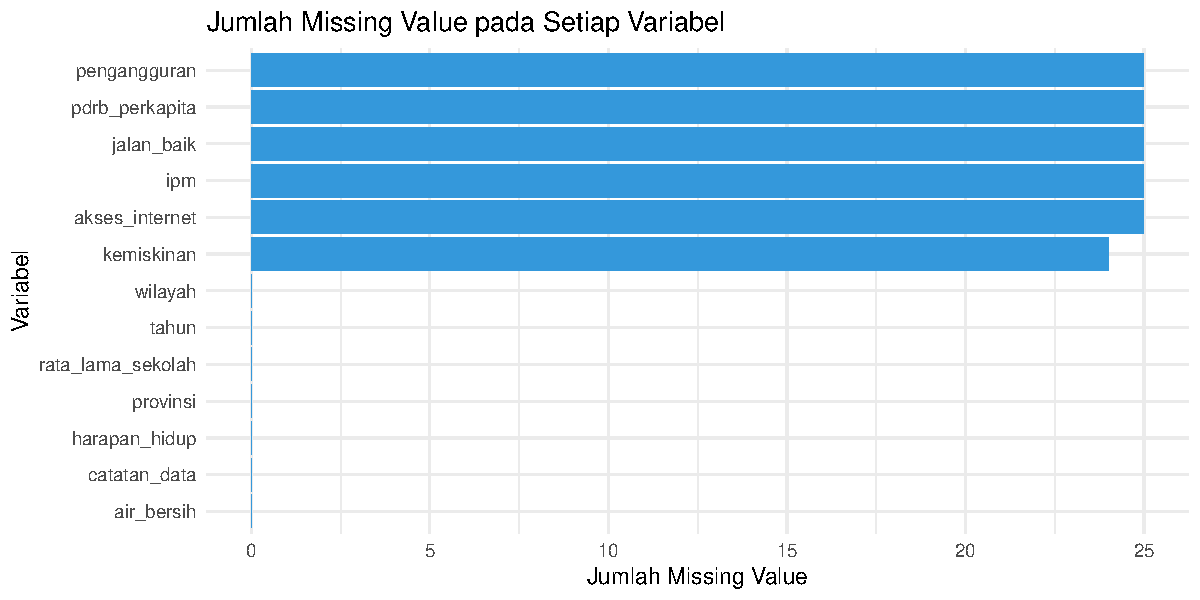
\includegraphics[keepaspectratio]{laporan_akhir_files/figure-pdf/unnamed-chunk-4-1.pdf}}

\begin{Shaded}
\begin{Highlighting}[]
\CommentTok{\# Menyimpan grafik ke dalam folder gambar}
\FunctionTok{ggsave}\NormalTok{(}
  \AttributeTok{filename =} \StringTok{"../gambar/gambar\_1\_missing\_value\_variabel.png"}\NormalTok{,}
  \AttributeTok{plot =}\NormalTok{ plot\_missing,}
  \AttributeTok{width =} \DecValTok{8}\NormalTok{,}
  \AttributeTok{height =} \DecValTok{4}\NormalTok{,}
  \AttributeTok{dpi =} \DecValTok{300}
\NormalTok{)}
\end{Highlighting}
\end{Shaded}

Berdasarkan Gambar 1, terlihat bahwa missing value tidak hanya terdapat
pada variabel utama, tetapi juga muncul pada beberapa variabel lain
dalam dataset. Grafik ini digunakan untuk melihat kondisi kelengkapan
data secara umum. Namun, karena analisis difokuskan pada hubungan antara
akses internet dan IPM, proses imputasi hanya dilakukan pada variabel
\texttt{akses\_internet} dan \texttt{ipm}.

\subsubsection{3.4.2 Grafik Jumlah Data Berdasarkan Catatan
Data}\label{grafik-jumlah-data-berdasarkan-catatan-data}

Grafik catatan data digunakan untuk melihat jumlah data berdasarkan
kategori yang tersedia pada kolom \texttt{catatan\_data}. Visualisasi
ini membantu mengetahui berapa banyak data yang termasuk normal, missing
value, maupun outlier.

\begin{Shaded}
\begin{Highlighting}[]
\CommentTok{\# Membuat data jumlah berdasarkan catatan\_data}
\NormalTok{catatan\_df }\OtherTok{\textless{}{-}} \FunctionTok{as.data.frame}\NormalTok{(}\FunctionTok{table}\NormalTok{(data}\SpecialCharTok{$}\NormalTok{catatan\_data))}
\FunctionTok{colnames}\NormalTok{(catatan\_df) }\OtherTok{\textless{}{-}} \FunctionTok{c}\NormalTok{(}\StringTok{"catatan\_data"}\NormalTok{, }\StringTok{"jumlah"}\NormalTok{)}

\CommentTok{\# Membuat grafik catatan data}
\NormalTok{plot\_catatan }\OtherTok{\textless{}{-}} \FunctionTok{ggplot}\NormalTok{(catatan\_df, }\FunctionTok{aes}\NormalTok{(}\AttributeTok{x =}\NormalTok{ catatan\_data, }\AttributeTok{y =}\NormalTok{ jumlah)) }\SpecialCharTok{+}
  \FunctionTok{geom\_col}\NormalTok{(}\AttributeTok{fill =} \StringTok{"\#e67e22"}\NormalTok{) }\SpecialCharTok{+}
  \FunctionTok{labs}\NormalTok{(}
    \AttributeTok{title =} \StringTok{"Jumlah Data Berdasarkan Catatan Data"}\NormalTok{,}
    \AttributeTok{x =} \StringTok{"Catatan Data"}\NormalTok{,}
    \AttributeTok{y =} \StringTok{"Jumlah Data"}
\NormalTok{  ) }\SpecialCharTok{+}
  \FunctionTok{theme\_minimal}\NormalTok{()}

\CommentTok{\# Menampilkan grafik pada laporan}
\NormalTok{plot\_catatan}
\end{Highlighting}
\end{Shaded}

\pandocbounded{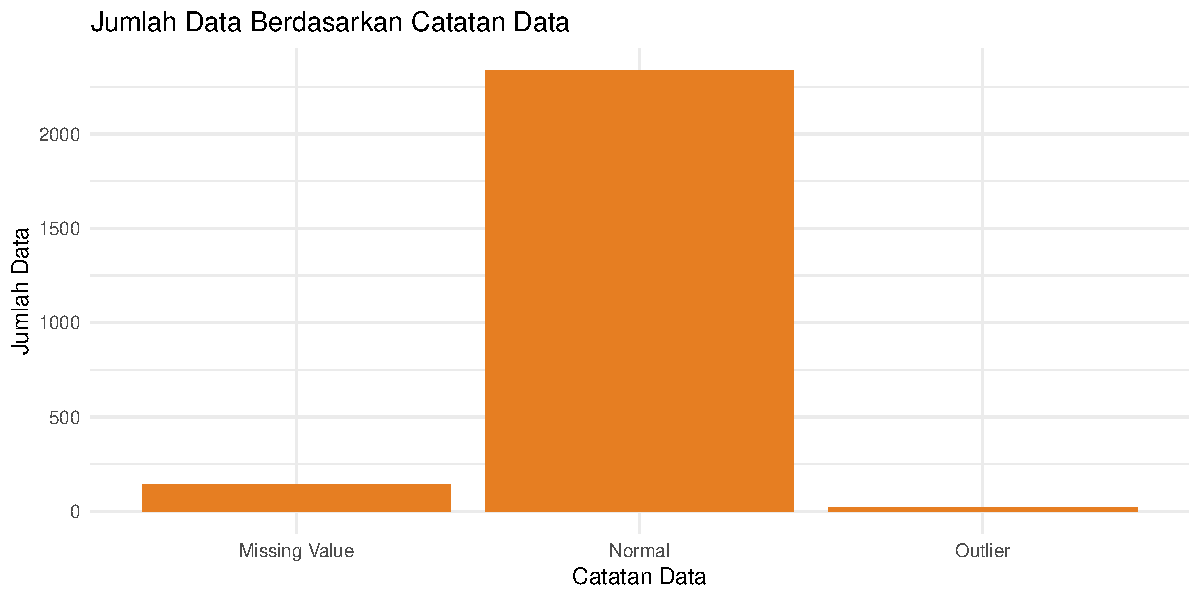
\includegraphics[keepaspectratio]{laporan_akhir_files/figure-pdf/unnamed-chunk-5-1.pdf}}

\begin{Shaded}
\begin{Highlighting}[]
\CommentTok{\# Menyimpan grafik ke dalam folder gambar}
\FunctionTok{ggsave}\NormalTok{(}
  \AttributeTok{filename =} \StringTok{"../gambar/gambar\_2\_catatan\_data.png"}\NormalTok{,}
  \AttributeTok{plot =}\NormalTok{ plot\_catatan,}
  \AttributeTok{width =} \DecValTok{8}\NormalTok{,}
  \AttributeTok{height =} \DecValTok{4}\NormalTok{,}
  \AttributeTok{dpi =} \DecValTok{300}
\NormalTok{)}
\end{Highlighting}
\end{Shaded}

Berdasarkan Gambar 2, sebagian besar data berada pada kategori normal,
sedangkan sebagian kecil data memiliki catatan missing value dan
outlier. Grafik ini menunjukkan bahwa dataset memang memiliki beberapa
catatan kualitas data yang perlu diperhatikan. Pada penelitian ini,
outlier tetap dipertahankan karena analisis difokuskan untuk melihat
hubungan umum antara akses internet dan IPM.

\subsubsection{3.4.3 Scatter Plot Hubungan Akses Internet dan
IPM}\label{scatter-plot-hubungan-akses-internet-dan-ipm}

Scatter plot digunakan untuk melihat pola hubungan antara tingkat akses
internet dan IPM. Visualisasi ini membantu menunjukkan apakah kenaikan
akses internet cenderung diikuti oleh kenaikan IPM atau tidak.

\begin{Shaded}
\begin{Highlighting}[]
\CommentTok{\# Membuat scatter plot hubungan akses internet dan IPM}
\NormalTok{plot\_scatter }\OtherTok{\textless{}{-}} \FunctionTok{ggplot}\NormalTok{(data, }\FunctionTok{aes}\NormalTok{(}\AttributeTok{x =}\NormalTok{ akses\_internet, }\AttributeTok{y =}\NormalTok{ ipm)) }\SpecialCharTok{+}
  \FunctionTok{geom\_point}\NormalTok{(}\AttributeTok{color =} \StringTok{"\#2980b9"}\NormalTok{, }\AttributeTok{alpha =} \FloatTok{0.5}\NormalTok{) }\SpecialCharTok{+}
  \FunctionTok{geom\_smooth}\NormalTok{(}\AttributeTok{method =} \StringTok{"lm"}\NormalTok{, }\AttributeTok{color =} \StringTok{"\#e74c3c"}\NormalTok{, }\AttributeTok{se =} \ConstantTok{TRUE}\NormalTok{) }\SpecialCharTok{+}
  \FunctionTok{labs}\NormalTok{(}
    \AttributeTok{title =} \StringTok{"Hubungan Akses Internet dan IPM"}\NormalTok{,}
    \AttributeTok{x =} \StringTok{"Akses Internet (\%)"}\NormalTok{,}
    \AttributeTok{y =} \StringTok{"IPM"}
\NormalTok{  ) }\SpecialCharTok{+}
  \FunctionTok{theme\_minimal}\NormalTok{()}

\CommentTok{\# Menampilkan plot pada laporan}
\NormalTok{plot\_scatter}
\end{Highlighting}
\end{Shaded}

\begin{verbatim}
`geom_smooth()` using formula = 'y ~ x'
\end{verbatim}

\pandocbounded{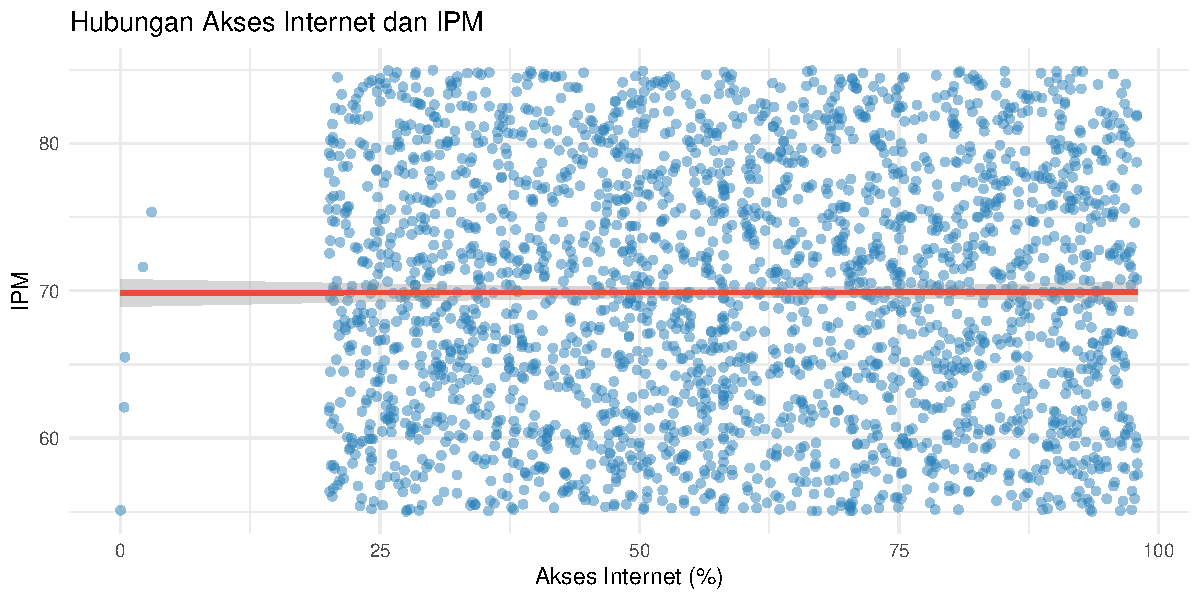
\includegraphics[keepaspectratio]{laporan_akhir_files/figure-pdf/unnamed-chunk-6-1.pdf}}

\begin{Shaded}
\begin{Highlighting}[]
\CommentTok{\# Menyimpan plot ke dalam folder gambar}
\FunctionTok{ggsave}\NormalTok{(}
  \AttributeTok{filename =} \StringTok{"../gambar/gambar\_3\_scatter\_akses\_internet\_ipm.png"}\NormalTok{,}
  \AttributeTok{plot =}\NormalTok{ plot\_scatter,}
  \AttributeTok{width =} \DecValTok{8}\NormalTok{,}
  \AttributeTok{height =} \DecValTok{4}\NormalTok{,}
  \AttributeTok{dpi =} \DecValTok{300}
\NormalTok{)}
\end{Highlighting}
\end{Shaded}

\begin{verbatim}
`geom_smooth()` using formula = 'y ~ x'
\end{verbatim}

Berdasarkan Gambar 3, titik-titik data terlihat menyebar secara acak dan
tidak membentuk pola naik atau turun yang jelas. Garis regresi pada
grafik juga hampir datar, sehingga hubungan linear antara akses internet
dan IPM belum terlihat kuat secara visual.

Dari visualisasi ini, dapat dikatakan bahwa wilayah dengan akses
internet yang lebih tinggi tidak selalu memiliki IPM yang lebih tinggi
dalam dataset ini. Oleh karena itu, hasil scatter plot perlu diperkuat
dengan uji korelasi Pearson untuk mengetahui apakah hubungan kedua
variabel signifikan secara statistik.

\subsubsection{3.4.4 Histogram Distribusi
IPM}\label{histogram-distribusi-ipm}

Histogram digunakan untuk melihat bentuk distribusi nilai IPM pada
dataset. Visualisasi ini membantu memberikan gambaran awal mengenai
apakah data IPM cenderung menyebar secara normal atau tidak sebelum
dilakukan uji normalitas.

\begin{Shaded}
\begin{Highlighting}[]
\CommentTok{\# Membuat histogram untuk melihat distribusi nilai IPM}
\NormalTok{plot\_histogram\_ipm }\OtherTok{\textless{}{-}} \FunctionTok{ggplot}\NormalTok{(data, }\FunctionTok{aes}\NormalTok{(}\AttributeTok{x =}\NormalTok{ ipm)) }\SpecialCharTok{+}
  \FunctionTok{geom\_histogram}\NormalTok{(}\AttributeTok{bins =} \DecValTok{30}\NormalTok{, }\AttributeTok{fill =} \StringTok{"\#3498db"}\NormalTok{, }\AttributeTok{color =} \StringTok{"white"}\NormalTok{) }\SpecialCharTok{+}
  \FunctionTok{labs}\NormalTok{(}
    \AttributeTok{title =} \StringTok{"Distribusi Nilai IPM"}\NormalTok{,}
    \AttributeTok{x =} \StringTok{"IPM"}\NormalTok{,}
    \AttributeTok{y =} \StringTok{"Frekuensi"}
\NormalTok{  ) }\SpecialCharTok{+}
  \FunctionTok{theme\_minimal}\NormalTok{()}

\CommentTok{\# Menampilkan histogram IPM pada laporan}
\NormalTok{plot\_histogram\_ipm}
\end{Highlighting}
\end{Shaded}

\pandocbounded{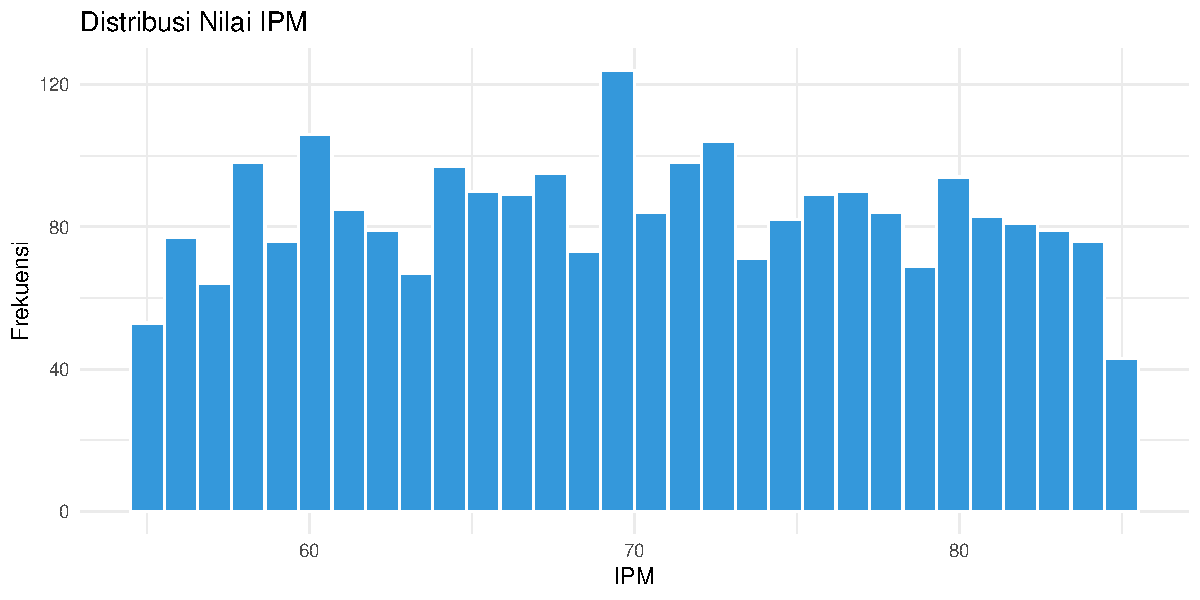
\includegraphics[keepaspectratio]{laporan_akhir_files/figure-pdf/unnamed-chunk-7-1.pdf}}

\begin{Shaded}
\begin{Highlighting}[]
\CommentTok{\# Menyimpan histogram IPM ke dalam folder gambar}
\FunctionTok{ggsave}\NormalTok{(}
  \AttributeTok{filename =} \StringTok{"../gambar/gambar\_4\_histogram\_ipm.png"}\NormalTok{,}
  \AttributeTok{plot =}\NormalTok{ plot\_histogram\_ipm,}
  \AttributeTok{width =} \DecValTok{8}\NormalTok{,}
  \AttributeTok{height =} \DecValTok{4}\NormalTok{,}
  \AttributeTok{dpi =} \DecValTok{300}
\NormalTok{)}
\end{Highlighting}
\end{Shaded}

Berdasarkan Gambar 4, nilai IPM tersebar pada beberapa rentang nilai dan
tidak sepenuhnya membentuk pola lonceng yang simetris. Hal ini
menunjukkan bahwa distribusi IPM perlu diperiksa lebih lanjut sebelum
digunakan dalam pengujian statistik.

Histogram ini hanya digunakan sebagai gambaran awal untuk melihat bentuk
sebaran data. Keputusan mengenai normal atau tidaknya distribusi IPM
tetap didasarkan pada hasil uji Shapiro-Wilk pada bagian berikutnya.

\subsubsection{3.4.5 Boxplot Akses Internet dan
IPM}\label{boxplot-akses-internet-dan-ipm}

Boxplot digunakan untuk melihat sebaran data, nilai tengah, rentang
data, serta kemungkinan adanya nilai ekstrem pada variabel akses
internet dan IPM.

\begin{Shaded}
\begin{Highlighting}[]
\CommentTok{\# Mengubah data akses internet dan IPM ke format panjang}
\NormalTok{data\_boxplot }\OtherTok{\textless{}{-}} \FunctionTok{data.frame}\NormalTok{(}
  \AttributeTok{variabel =} \FunctionTok{rep}\NormalTok{(}\FunctionTok{c}\NormalTok{(}\StringTok{"Akses Internet"}\NormalTok{, }\StringTok{"IPM"}\NormalTok{), }\AttributeTok{each =} \FunctionTok{nrow}\NormalTok{(data)),}
  \AttributeTok{nilai =} \FunctionTok{c}\NormalTok{(data}\SpecialCharTok{$}\NormalTok{akses\_internet, data}\SpecialCharTok{$}\NormalTok{ipm)}
\NormalTok{)}

\CommentTok{\# Membuat boxplot akses internet dan IPM}
\NormalTok{plot\_boxplot }\OtherTok{\textless{}{-}} \FunctionTok{ggplot}\NormalTok{(data\_boxplot, }\FunctionTok{aes}\NormalTok{(}\AttributeTok{x =}\NormalTok{ variabel, }\AttributeTok{y =}\NormalTok{ nilai, }\AttributeTok{fill =}\NormalTok{ variabel)) }\SpecialCharTok{+}
  \FunctionTok{geom\_boxplot}\NormalTok{(}\AttributeTok{alpha =} \FloatTok{0.7}\NormalTok{) }\SpecialCharTok{+}
  \FunctionTok{labs}\NormalTok{(}
    \AttributeTok{title =} \StringTok{"Boxplot Akses Internet dan IPM"}\NormalTok{,}
    \AttributeTok{x =} \StringTok{"Variabel"}\NormalTok{,}
    \AttributeTok{y =} \StringTok{"Nilai"}
\NormalTok{  ) }\SpecialCharTok{+}
  \FunctionTok{theme\_minimal}\NormalTok{() }\SpecialCharTok{+}
  \FunctionTok{theme}\NormalTok{(}\AttributeTok{legend.position =} \StringTok{"none"}\NormalTok{)}

\CommentTok{\# Menampilkan boxplot pada laporan}
\NormalTok{plot\_boxplot}
\end{Highlighting}
\end{Shaded}

\pandocbounded{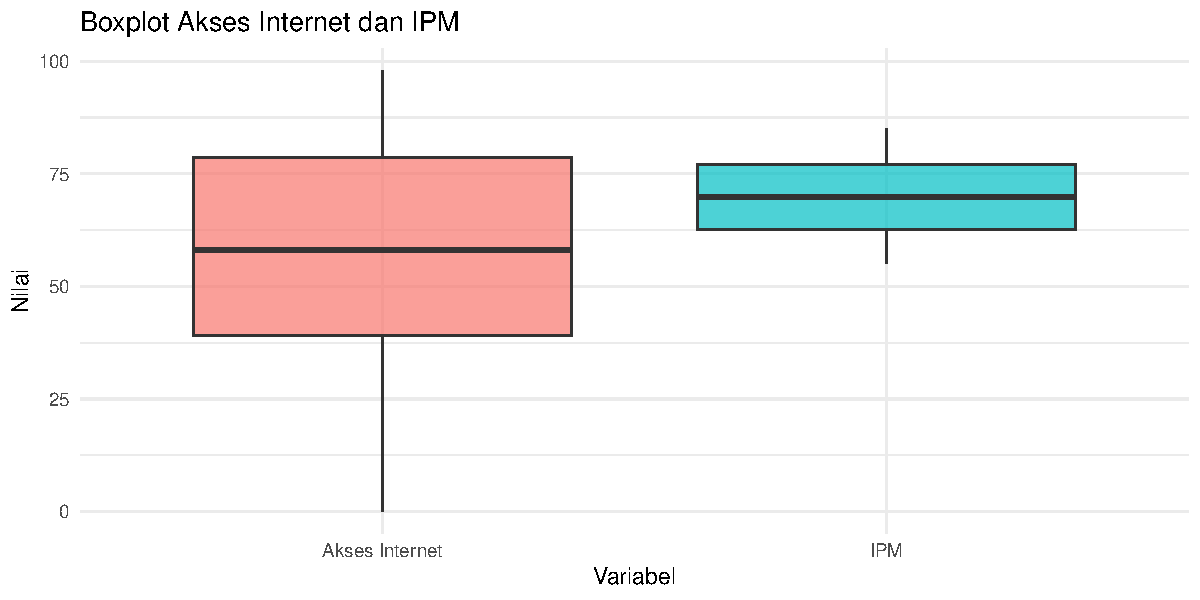
\includegraphics[keepaspectratio]{laporan_akhir_files/figure-pdf/unnamed-chunk-8-1.pdf}}

\begin{Shaded}
\begin{Highlighting}[]
\CommentTok{\# Menyimpan boxplot ke dalam folder gambar}
\FunctionTok{ggsave}\NormalTok{(}
  \AttributeTok{filename =} \StringTok{"../gambar/gambar\_5\_boxplot\_akses\_internet\_ipm.png"}\NormalTok{,}
  \AttributeTok{plot =}\NormalTok{ plot\_boxplot,}
  \AttributeTok{width =} \DecValTok{8}\NormalTok{,}
  \AttributeTok{height =} \DecValTok{4}\NormalTok{,}
  \AttributeTok{dpi =} \DecValTok{300}
\NormalTok{)}
\end{Highlighting}
\end{Shaded}

Berdasarkan Gambar 5, boxplot menunjukkan sebaran nilai pada variabel
akses internet dan IPM. Visualisasi ini membantu melihat nilai tengah,
rentang data, serta kemungkinan adanya nilai ekstrem. Jika terdapat
titik yang berada jauh dari kotak utama, maka titik tersebut dapat
menjadi indikasi outlier. Namun, outlier tetap dipertahankan karena
analisis ini berfokus pada hubungan umum antarvariabel, bukan pada
penghapusan data ekstrem.

\subsection{3.5 Uji Normalitas}\label{uji-normalitas}

Sebelum melakukan uji korelasi Pearson, perlu dipastikan bahwa data
memenuhi asumsi normalitas. Oleh karena itu, dilakukan Uji Shapiro-Wilk
pada variabel IPM.

\begin{Shaded}
\begin{Highlighting}[]
\NormalTok{shapiro\_test }\OtherTok{\textless{}{-}} \FunctionTok{shapiro.test}\NormalTok{(data}\SpecialCharTok{$}\NormalTok{ipm)}

\FunctionTok{cat}\NormalTok{(}\StringTok{"Hasil Uji Normalitas:}\SpecialCharTok{\textbackslash{}n}\StringTok{"}\NormalTok{)}
\end{Highlighting}
\end{Shaded}

\begin{verbatim}
Hasil Uji Normalitas:
\end{verbatim}

\begin{Shaded}
\begin{Highlighting}[]
\FunctionTok{print}\NormalTok{(shapiro\_test)}
\end{Highlighting}
\end{Shaded}

\begin{verbatim}

    Shapiro-Wilk normality test

data:  data$ipm
W = 0.96032, p-value < 2.2e-16
\end{verbatim}

Pada pengujian ini digunakan hipotesis sebagai berikut:

\begin{itemize}
\item
  H0 : Data berdistribusi normal.
\item
  H1 : Data tidak berdistribusi normal.
\end{itemize}

Berdasarkan hasil pengujian diperoleh nilai p-value \textless{} 0,05
sehingga H0 ditolak. Dengan demikian, data IPM tidak berdistribusi
normal.

Namun demikian, jumlah sampel yang digunakan cukup besar, yaitu sekitar
2.500 observasi. Pada ukuran sampel yang besar, penyimpangan kecil dari
distribusi normal sering kali membuat hasil uji normalitas menjadi
signifikan secara statistik (Ghasemi \& Zahediasl, 2012). Oleh karena
itu, uji korelasi Pearson tetap digunakan untuk melihat kecenderungan
hubungan linear antara akses internet dan IPM.

\subsection{3.6 Uji Korelasi Pearson}\label{uji-korelasi-pearson}

Tahap terakhir adalah menguji hubungan antara penetrasi akses internet
dan IPM menggunakan Uji Korelasi Pearson. Pengujian ini dilakukan untuk
mengetahui apakah terdapat hubungan yang signifikan antara kedua
variabel serta mengukur kekuatan hubungan tersebut.

\begin{Shaded}
\begin{Highlighting}[]
\NormalTok{korelasi\_test }\OtherTok{\textless{}{-}} \FunctionTok{cor.test}\NormalTok{(}
\NormalTok{  data}\SpecialCharTok{$}\NormalTok{akses\_internet,}
\NormalTok{  data}\SpecialCharTok{$}\NormalTok{ipm,}
  \AttributeTok{method =} \StringTok{"pearson"}
\NormalTok{)}

\FunctionTok{print}\NormalTok{(korelasi\_test)}
\end{Highlighting}
\end{Shaded}

\begin{verbatim}

    Pearson's product-moment correlation

data:  data$akses_internet and data$ipm
t = 0.10552, df = 2498, p-value = 0.916
alternative hypothesis: true correlation is not equal to 0
95 percent confidence interval:
 -0.03709453  0.04131056
sample estimates:
        cor 
0.002111257 
\end{verbatim}

Hipotesis yang digunakan adalah:

\begin{itemize}
\tightlist
\item
  H0 : Tidak terdapat hubungan yang signifikan antara akses internet dan
  IPM.
\item
  H1 : Terdapat hubungan yang signifikan antara akses internet dan IPM.
\end{itemize}

Berdasarkan hasil pengujian diperoleh nilai koefisien korelasi (r)
sebesar 0,0021 dengan p-value sebesar 0,916.

Nilai koefisien korelasi yang sangat mendekati nol menunjukkan bahwa
hubungan linear antara akses internet dan IPM hampir tidak ada. Selain
itu, nilai p-value yang jauh lebih besar dari 0,05 menunjukkan bahwa
hubungan tersebut tidak signifikan secara statistik.

Dengan demikian, H0 tidak ditolak sehingga tidak terdapat bukti yang
cukup untuk menyatakan adanya hubungan yang signifikan antara tingkat
akses internet dan IPM pada dataset yang dianalisis.

Hasil ini menunjukkan bahwa akses internet tidak memiliki hubungan
linear yang signifikan dengan IPM pada dataset yang dianalisis. Dengan
demikian, variasi IPM tidak dapat dijelaskan hanya melalui variabel
akses internet. Faktor lain seperti pendidikan, pendapatan, layanan
kesehatan, atau indikator pembangunan lainnya dapat menjadi bahan
pertimbangan untuk analisis lanjutan, tetapi tidak diuji secara langsung
dalam penelitian ini.

\section{BAB IV: KESIMPULAN}\label{bab-iv-kesimpulan}

\subsection{4.1 Kesimpulan Utama}\label{kesimpulan-utama}

Berdasarkan hasil analisis, missing value pada variabel
\texttt{akses\_internet} dan \texttt{ipm} berhasil ditangani menggunakan
Median Imputation. Analisis deskriptif menunjukkan bahwa nilai akses
internet dan IPM memiliki variasi antarwilayah. Lima visualisasi yang
dibuat juga membantu memperlihatkan kondisi missing value, catatan data,
pola hubungan, distribusi IPM, serta kemungkinan nilai ekstrem.

Hasil scatter plot menunjukkan bahwa hubungan antara akses internet dan
IPM tidak membentuk pola linear yang kuat. Selain itu, uji Shapiro-Wilk
menunjukkan bahwa data IPM tidak berdistribusi normal karena p-value
kurang dari 0,05.

Pada uji korelasi Pearson, diperoleh koefisien korelasi sebesar 0,0021
dengan p-value sebesar 0,916. Nilai tersebut menunjukkan bahwa hubungan
linear antara akses internet dan IPM sangat lemah dan tidak signifikan
secara statistik.

Secara keseluruhan, tingkat akses internet tidak memiliki hubungan
linear yang signifikan dengan IPM pada dataset yang digunakan dalam
penelitian ini.

\subsection{4.2 Insight}\label{insight}

Hasil analisis menunjukkan bahwa akses internet belum cukup kuat untuk
menjelaskan variasi IPM secara linear pada dataset ini. Artinya, wilayah
dengan akses internet yang lebih tinggi tidak selalu memiliki nilai IPM
yang lebih tinggi. Temuan ini menunjukkan bahwa pembangunan manusia
tidak dapat dilihat hanya dari satu indikator digital, tetapi perlu
mempertimbangkan indikator lain seperti pendidikan, kesehatan, ekonomi,
dan infrastruktur.

\subsection{4.3 Saran}\label{saran}

Untuk analisis lanjutan, disarankan menggunakan lebih banyak variabel
pembangunan seperti tingkat kemiskinan, pengangguran, PDRB per kapita,
rata-rata lama sekolah, harapan hidup, akses air bersih, dan kondisi
jalan baik. Analisis lanjutan juga dapat menggunakan korelasi antar
banyak variabel atau model regresi agar faktor-faktor yang berhubungan
dengan IPM dapat dipahami secara lebih luas.

\section{DAFTAR PUSTAKA}\label{daftar-pustaka}

Badan Pusat Statistik. (2023). \emph{Indeks Pembangunan Manusia 2023}.
Badan Pusat Statistik Republik Indonesia.

Field, A., Miles, J., \& Field, Z. (2012). \emph{Discovering Statistics
Using R}. SAGE Publications.

Ghasemi, A., \& Zahediasl, S. (2012). Normality tests for statistical
analysis: A guide for non-statisticians. \emph{International Journal of
Endocrinology and Metabolism, 10}(2), 486--489.

Little, R. J. A., \& Rubin, D. B. (2019). \emph{Statistical Analysis
with Missing Data} (3rd ed.). John Wiley \& Sons.

Ndubuisi, G., Otioma, C., \& Tetteh, G. K. (2021). Digital
infrastructure and human development. \emph{Telecommunications Policy,
45}(8), 102154.

United Nations Development Programme. (2022). \emph{Human Development
Report 2021/2022: Uncertain Times, Unsettled Lives}. United Nations
Development Programme.

\section{LAMPIRAN}\label{lampiran}

Lampiran berisi file pendukung yang digunakan dalam penyusunan laporan
proyek akhir ini.

\begin{enumerate}
\def\labelenumi{\arabic{enumi}.}
\tightlist
\item
  Script R disimpan pada folder \texttt{script}.
\item
  Dataset disimpan pada folder \texttt{dataset}.
\item
  Hasil visualisasi disimpan pada folder \texttt{gambar}.
\item
  Laporan akhir dalam format \texttt{.qmd} dan \texttt{.pdf} disimpan
  pada folder \texttt{dokumen}.
\end{enumerate}

Adapun hasil visualisasi yang disimpan pada folder \texttt{gambar}
adalah:

\begin{enumerate}
\def\labelenumi{\arabic{enumi}.}
\tightlist
\item
  \texttt{gambar\_1\_missing\_value\_variabel.png}
\item
  \texttt{gambar\_2\_catatan\_data.png}
\item
  \texttt{gambar\_3\_scatter\_akses\_internet\_ipm.png}
\item
  \texttt{gambar\_4\_histogram\_ipm.png}
\item
  \texttt{gambar\_5\_boxplot\_akses\_internet\_ipm.png}
\end{enumerate}




\end{document}
